\documentclass[a4paper]{article}

%% Language and font encodings
\usepackage[english]{babel}
\usepackage[utf8x]{inputenc}
\usepackage[T1]{fontenc}
\usepackage{amsmath}
\newcommand\norm[1]{\left\lVert#1\right\rVert}

%% Sets page size and margins
\usepackage[a4paper,top=3cm,bottom=2cm,left=3cm,right=3cm,marginparwidth=1.75cm]{geometry}

%% Useful packages
%%%%%%%%% begin snippet
%% You need to add the package "tabularx".
%% Place the snippet right after \begin{document}

% need tabularx
\usepackage{tabularx}
\usepackage{amsmath}
\usepackage{graphicx}
\usepackage[colorinlistoftodos]{todonotes}
\usepackage{paralist}
\usepackage{amssymb,amsmath,amsthm,enumitem}
\usepackage[colorlinks=true, allcolors=blue]{hyperref}
\usepackage{subcaption}
\setlength{\abovedisplayskip}{3pt}
\setlength{\belowdisplayskip}{3pt}
\usepackage[hypcap=false]{caption}

\captionsetup{justification=centering}
\captionsetup{format=plain, font=small, labelfont=bf}

\begin{document}
\title{ Computational Intelligence, SS2018 Assignment 5}

\begin{titlepage}
       \begin{center}
             \begin{huge}
				   %% Update assignment number here
                   \textbf{Assignment 5}
             \end{huge}
       \end{center}

       \begin{center}
             \begin{large}
                   Computational Intelligence, SS2018
             \end{large}
       \end{center}

       \begin{center}
 \begin{tabularx}{\textwidth}{|>{\hsize=.33\hsize}X|>{\hsize=.33\hsize}X|>{\hsize=.33\hsize}X|} 

                   \hline
                   \multicolumn{3}{|c|}{\textbf{Team Members}} \\
                   \hline
                   STRUGER & Patrick & 01530664 \\
                   \hline
                   B\"OCK & Manfred & 01530598 \\
                   \hline
                   HAUPT & Anna & 01432018 \\
                   \hline

             \end{tabularx}
       \end{center}

\end{titlepage}

%%%%%%%%% end snippet 

\newpage
\tableofcontents
\newpage

\section{Background}
This section explains the algorithms that have to be implemented. The actual tasks are provided in the subsequent sections.

\subsection{Expectation Maximization Algorithm}

\begin{enumerate}
\item Write a function that implements the EM algorithm: \\
$alpha, mean, cov, LL, labels = EM(X, K, alpha\_0, mu\_0, sigma\_0, max\_iter, tol).$\\
Here, $X$ is the data set and consists of $N = 150$ samples. $K$ is the number of Gaussian components. The initial parameter vector is $alpha\_0$, $mean\_0$, and $cov\_0$. The maximum number of iterations and the tolerance are given by $max iter$ and $tol$. After convergence the function returns the final parameter vector given by alpha, mu, and cov, as well as the log-likelihood over the iterations in LL. The function further returns the labels that
are obtained by performing soft classification of each sample according to (2) 
\newline
You may use the provided function $P = likelihood\_multivariate\_normal(X,mu,cov,log)$ that estimates the likelihood, or the log-likelihood, of $X$ given the specified multivariate Gaussian distribution.
\end{enumerate}

\subsection{K-means algorithm}
You should implement the K-means algorithm as discussed in the lecture and compare the results with the ones obtained with the EM-algorithm. Remember that you can interpret K-means as a version of the EM-algorithm with several simplifications: First, the classes are just represented by their means, second, there are no class weights and third, a hard classification is performed for all samples. The latter also means that for the parameter update, only the points classified to this component play a role.
\begin{enumerate}
\item  Write a function $centers\_0 = init\_k\_means(dimension, nr\_clusters, scenario)$ that provides the initial cluster centers centers\_0.
\item Further write a function that implements the K-means algorithm: $centers, D, labels = k\_means(X, K, centers\_0, max\_iter, tol)$\\
Here, $X$ is the data, $K$ is the number of clusters, centers\_0 are the initial cluster centers and max\_iter and tol are the maximum number of iterations and the tolerance. The function returns the optimized cluster centers centers and the cumulative distance over the iterations in $D$. All labels are obtained by performing hard classification for each sample.
\end{enumerate}


\subsection{Principal Component Analysis (PCA)}
You should also implement PCA as discussed in the lecture and apply it to reduce the dimension of the data from $D = 4$ to $M = 2$.
\begin{enumerate}
  \item Write a function $Y,V = PCA(data, M, whitening)$ that computes the first $M$ principal components and transforms the data, so that $y_n = U^T x_n$. The function should further return V that explains the amount of variance that is explained by the transformation.
  \item (bonus-task) If different features are on different scales it can be an important preprocessing step to transform the data such that $Y$ has zero mean and a covariance matrix equal to the identity matrix. Implement this and perform the according transformation if $whitening = True$.
\end{enumerate}

\newpage

\section{Classification/ Clustering}
We use three different scenarios (Sec. 2.1- 2.3) in order to evaluate the EM- and the K-means algorithm. Each scenario uses a different pre-processing step before applying the algorithms. Test your EM-algorithm for all three scenarios:

\begin{enumerate}
  \item Compare the result with the labeled data set (i.e., consider labels as well). Make a scatter plot of the data and plot the Gaussian mixture model over this plot. You can use the provided function plot\_gauss\_contour(mu,cov,xmin,xmax,ymin,ymax,nr\_points,title) for plotting each of the Gaussian components. The factors $\alpha_k$ are neglected for the visualization. Make sure to choose an appropriate range for plotting.  
  
\item your tests, select the correct number of components (K = 3), but also check the result when you use more or less components. How do you choose your initialization $\Theta_0$? Does this choice have an influence on the result?
  
\item Also plot the log-likelihood function over the iterations! What is the behavior of this function over the iterations?

\item Make a scatter plot of the data that shows the result of the soft-classification that is done in the E-step. Therefore classify each sample using $r^n_k$, and plot the samples in different colors for each of the three classes. You may use the provided functions plot\_iris\_data(data,labels) and reassign\_class\_labels(labels) in order to produce comparable plots.
\end{enumerate}

Further apply and evaluate your K-means algorithm for all three scenarios:
\begin{enumerate}[resume]
\item Perform the same tasks as for the EM-algorithm to evaluate the performance! The way to plot the classes/components is different now: in the scatter plot, plot the mean value for each class and plot the points classified to this class in a certain color.

\item  What is the nature of the boundaries between the classes? Compare with the results of the soft-classification in the EM-algorithm! Also compare with the labeled data, can K-means find the class structure well? \\

The nature boundaries between the classes is mainly linear. This is also the reason why our k-mean performs very well concerning our classification while the EM algorithm uses the gaussian shape for its Gaussian mixture models which was not as good as the k-mean performance. The k-mean algorithm classifies the data set linear with the minimum distance of its centers.
\end{enumerate}

\newpage

\subsection{2 dimensional feature [14 + 2* Points]}
In this scenario we consider only two of the available features (sepal length and petal length), i.e., x\_2dim.
\begin{enumerate}

\item \textbf{Perform all of the above-mentioned tasks for the EM algorithm. [7 Points]} \\

{\large \textbf{Comparing Standard Dataset with Gaussian Mixture Model}} \\

%%%%%%%%%%%%%%%%% Gaussian Mixture Model %%%%%%%%%%%%%%%%%
  
\begin{figure}[htp]
\centering
\begin{minipage}{0.4\textwidth}
  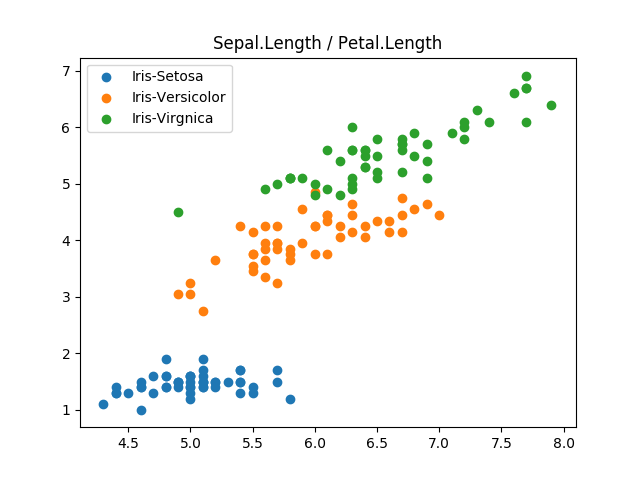
\includegraphics[scale=0.5]{plots/basic_scenario1_cmpnt3.png}
  \captionof{figure}{Standard data set (2dim).}
  \label{fig:16}
\end{minipage}
\hfill
\begin{minipage}{0.4\textwidth}
  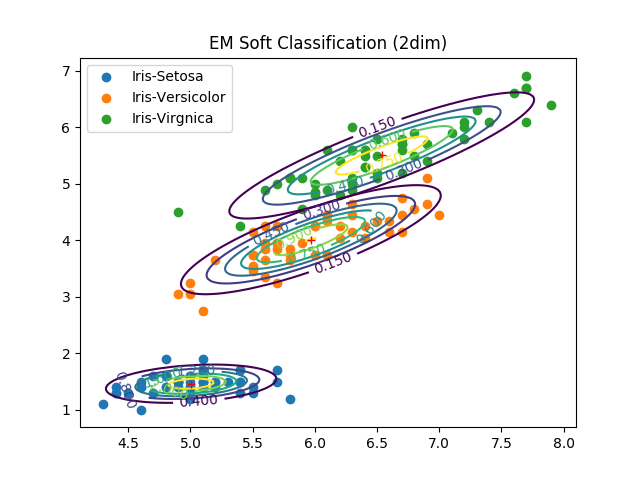
\includegraphics[scale=0.5]{plots/soft_classification_scenario1_cmpnt3.png}
  \captionof{figure}{Gaussian mixture model.}
  \label{fig:17}
\end{minipage}
\end{figure} 

In general we used the Expectation Maxmimization Algorithm (EM) to calculate our gaussian mixture model with the initialization values of mean, $\Theta$ and the covariance matrix. The initial values depend on random values in between the range of the values of the standard data set. The EM algorithm is used to learn gaussian mixture models which is done iteratively with the initial values mentioned before. This is done iteratively until the log-likelihood function converged. For a detailed explanation of the components and their calculation have a look at the background section above. As shown in the figure above, the gaussian mixture model classifies the data set very well but with little variance. A few values of the data set of the \textit{Iris-Versicolor} are classified as values of the \textit{Iris-Virgnica} dataset and vice versa. The data of \textit{Iris-Setosa} are well classified. \\
\newpage
{\large \textbf{Comparing with different Component Numbers}} \\

%%%%%%%%%%%%%%%%% Component Numbers %%%%%%%%%%%%%%%%%

\begin{figure}[htp]
\centering
\begin{minipage}{0.4\textwidth}
  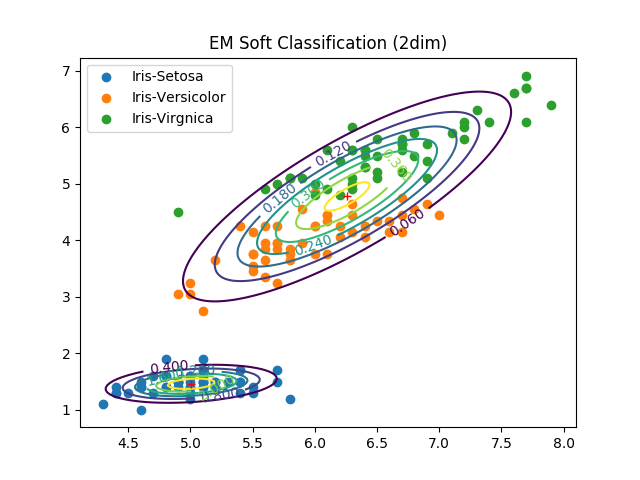
\includegraphics[scale=0.5]{plots/gauss_sc1_c2.png}
  \captionof{figure}{Gaussian mixture model with 2 components.}
  \label{fig:16}
\end{minipage}
\hfill
\begin{minipage}{0.4\textwidth}
  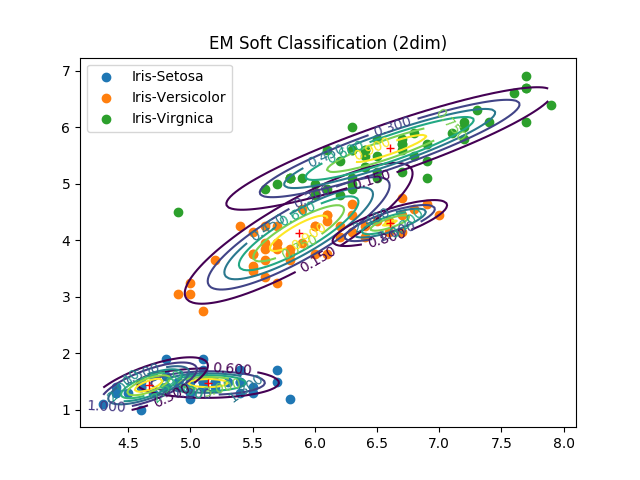
\includegraphics[scale=0.5]{plots/gauss_sc1_c5.png}
  \captionof{figure}{Gaussian mixture model with 5 components.}
  \label{fig:17}
\end{minipage}
\end{figure}

In this plots we can see the difference when using the standard 2-dimensional dataset with 2 components and when using 5 components.
When using the 2 components the EM classifies the data set as expected because \textit{Iris-Versicolor} and \textit{Iris-Virgnica} are really nearby and therefore they are classified as one set. On the other hand we have the model with 5 components both, the \textit{Iris-Sentosa} and the \textit{Iris-Versicolor} are split up into two classes while the values of \textit{Iris-Virgnica} are mainly in their whole regular class. The initialization of \textbf{$\Theta$ plays a key role} since it is the inverse value of the amount of components. \\

{\large \textbf{Log Likelihood over Iterations}} \\

%%%%%%%%%%%%%%%%% Log Likelihood %%%%%%%%%%%%%%%%%

\begin{figure}[htp]
\centering
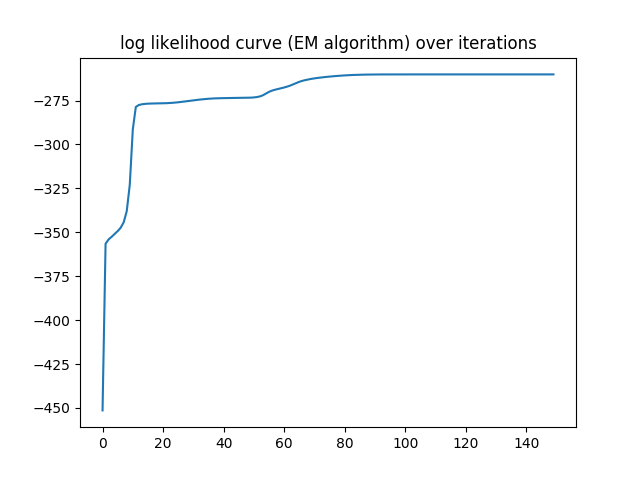
\includegraphics[scale=0.5]{plots/LL_scenario1_cmpnt3.png}
  \captionof{figure}{log-likelihood function over the iterations.}
  \label{fig:17}
\end{figure}

The log-likelihood function is used to calculate the probability of a parameter of our model, with the given initial values. As shown in the figure above the log-likelihood is increasing over the numbers of iterations by summing up the individual log-likelihood probabilities. It doesn't change that much after a certain point of iterations (in our case around 70 iterations). The EM algorithm finds local maximas which means a local maxima of the likelihood function. In our implementation the local maxima stays around at a value of -273.\newline

\newpage
{\large \textbf{Scatter Plot with Soft Classification}} \\

%%%%%%%%%%%%%%%%% Scatter Plot %%%%%%%%%%%%%%%%%

\begin{figure}[htp]
\begin{minipage}{0.4\textwidth}
	\centering
  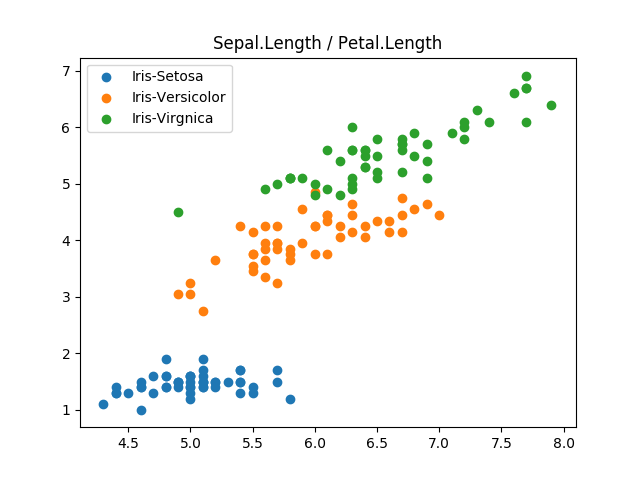
\includegraphics[scale=0.6]{plots/basic_scenario1_cmpnt3.png}
  \caption{Standard data set.}
\end{minipage}
\hfill
\begin{minipage}{0.4\textwidth}
	\centering
  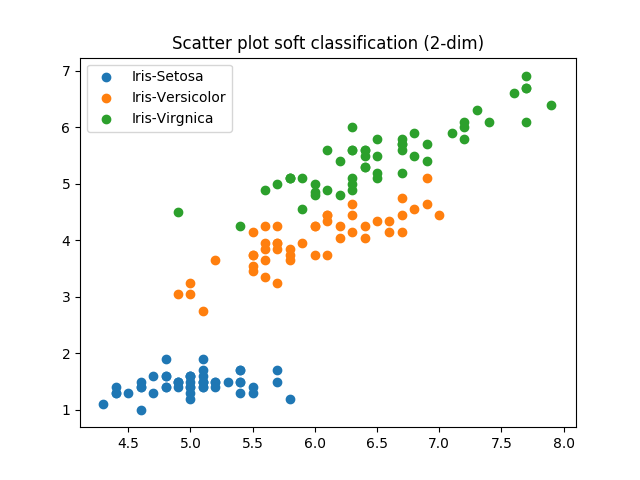
\includegraphics[scale=0.6]{plots/soft_scatter_scenario1_cmpnt3.png}
  \caption{Soft-classification.}
\end{minipage}
\end{figure}

In the scatter plot we now can see in detail which of the data points are classified as they should and which are not. The cluster classification of the \textit{Iris-Setosa} is classified perfectly, which means that every data point is classified as it should be.
But there are a few data points of the \textit{Iris-Versicolor} are classified as values of the \textit{Iris-Virgnica} dataset and vice versa. But the soft classification is still very reliable.

\newpage

\item \textbf{Perform all of the above-mentioned tasks for the K-means algorithm. [7 Points]} \\ \newline
The K-Means algorithm can be considered as a simplification of the EM algorithm. For the choice of starting points random points from the given data set were used. After that, each sample was assigned a center (smallest distance) $\Rightarrow$ Classification of the samples to the components (modified E-step).
Then the centers were recalculated. This was done until the newly calculated centers differed only very slightly from the old ones or the maximum number of iterations was reached.
\newline
\newline
{\large \textbf{Comparing Standard Dataset with K-mean Model}} \\

%%%%%%%%%%%%%%%%% K-mean Model %%%%%%%%%%%%%%%%%
  
\begin{figure}[htp]
\centering
\begin{minipage}{0.4\textwidth}
  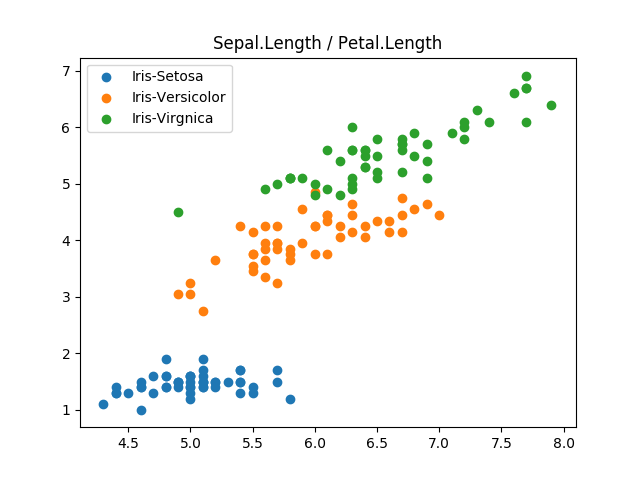
\includegraphics[scale=0.5]{plots/basic_scenario1_cmpnt3.png}
  \captionof{figure}{Standard data set.}
  \label{fig:16}
\end{minipage}
\hfill
\begin{minipage}{0.4\textwidth}
  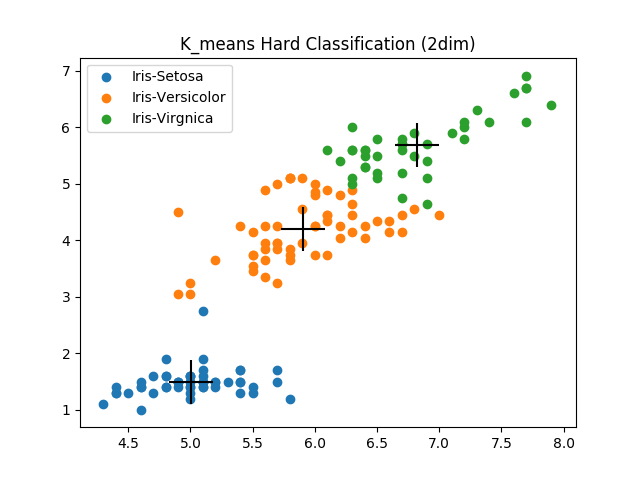
\includegraphics[scale=0.5]{plots/hard_classification_scenario1_cmpnt3.png}
  \captionof{figure}{K-mean model.}
  \label{fig:17}
\end{minipage}
\end{figure} 
The classification works quite well when testing the K-Mean algorithm with three clusters. The centers converge always to the largest collections of points. That means that the \textit{Iris-Sentosa}, the \textit{Iris-Versicolor} \& the \textit{Iris-Virgnica} contain one center each. \\

\newpage

{\large \textbf{Comparing with different Component Numbers}} \\

%%%%%%%%%%%%%%%%% Component Numbers %%%%%%%%%%%%%%%%%

\begin{figure}[htp]
\centering
\begin{minipage}{0.4\textwidth}
  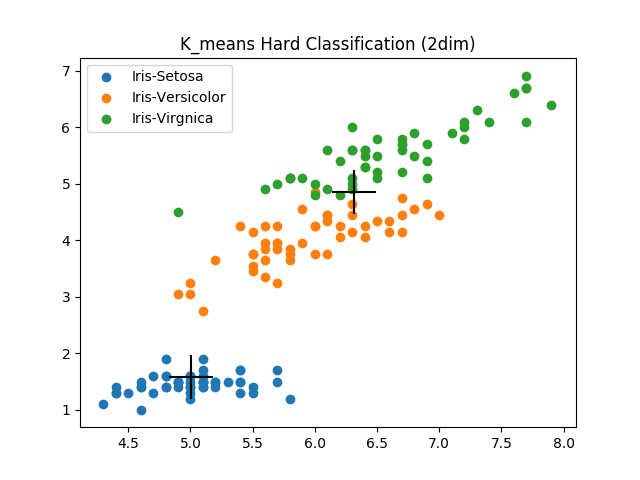
\includegraphics[scale=0.5]{plots/kmeans_sc1_c2.png}
  \captionof{figure}{K-mean model with 2 components.}
  \label{fig:16}
\end{minipage}
\hfill
\begin{minipage}{0.4\textwidth}
  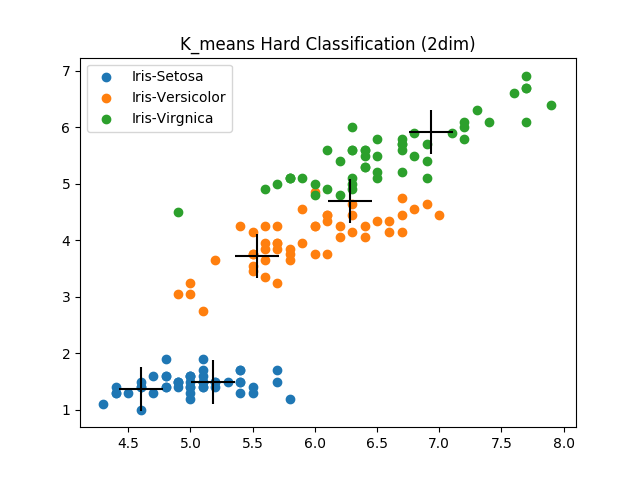
\includegraphics[scale=0.5]{plots/kmeans_sc1_c5.png}
  \captionof{figure}{K-mean model with 5 components.}
  \label{fig:17}
\end{minipage}
\end{figure} 

Testing the K-Mean algorithm with two \& five clusters showed that when using two clusters, one center converge to the midpoint between \textit{Iris-Versicolor} \& \textit{Iris-Virgnica}, because this two sets are really close to each other and therefore they are classified as one set. But when using 5 clusters, the \textit{Iris-Sentosa} contains two centers while both the \textit{Iris-Virgnica} \& the \textit{Iris-Versicolor} contain only one center. Last center is between the \textit{Iris-Virgnica} \& the \textit{Iris-Versicolor}.\\

{\large \textbf{Cumulative Distance over Iterations}} \\

%%%%%%%%%%%%%%%%% Cumulative Distance %%%%%%%%%%%%%%%%%

\begin{figure}[htp]
\centering
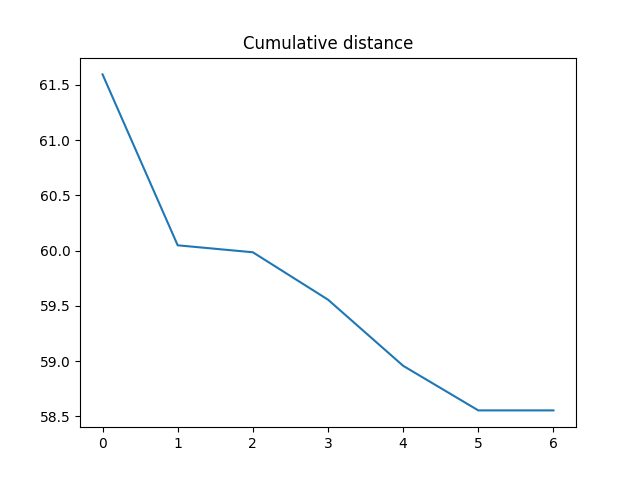
\includegraphics[scale=0.5]{plots/CC_scenario1_cmpnt3.png}
  \captionof{figure}{Cumulative distance over the iterations.}
  \label{fig:17}
\end{figure}

K-means converged to the local minima of the cumulative distance. The result depends on the initialization of $\Theta$ which means that it won't found a global optimum regularly. Decisions between the cluster are partly linear which is also shown in the figure above. The cumulative distance is decreasing over the numbers of iterations. We used random initial values for the k-mean algorithm (same as in EM). The result strongly depends on the initial values. The classification with our k-mean found some local minima while using 3 components. After 6 iterations the local minima stays steady at a value between 58.5 and 59. \newline \newline

\newpage

{\large \textbf{Scatter Plot with Hard Classification}} \\

%%%%%%%%%%%%%%%%% Scatter Plot %%%%%%%%%%%%%%%%%

\begin{figure}[htp]
\begin{minipage}{0.4\textwidth}
	\centering
  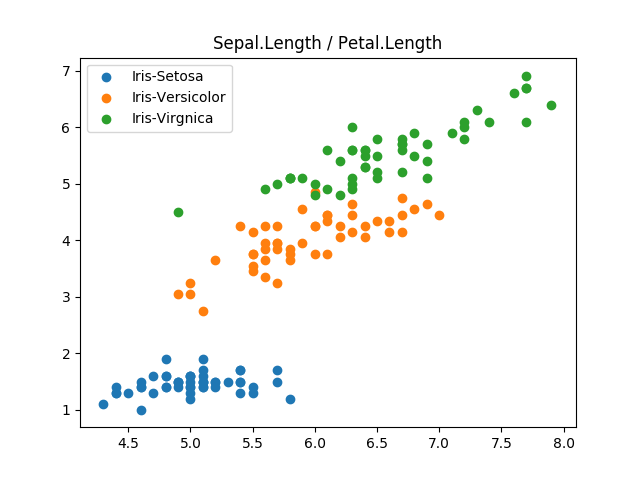
\includegraphics[scale=0.6]{plots/basic_scenario1_cmpnt3.png}
  \caption{Standard data set.}
\end{minipage}
\hfill
\begin{minipage}{0.4\textwidth}
	\centering
  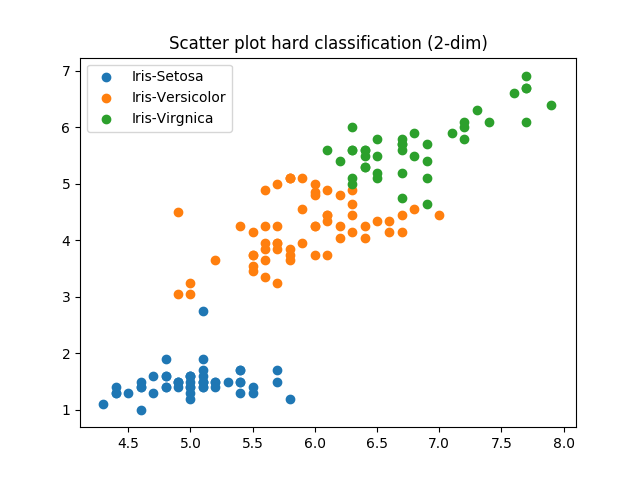
\includegraphics[scale=0.6]{plots/hard_scatter_scenario1_cmpnt3.png}
  \caption{Hard-classification.}
\end{minipage}
\end{figure}

The k-mean classification in D = 2 is able to classify most of the components well. The \textit{Iris-Setosa} is classified perfectly while Iris-Versicolor got some data from Iris-Virgnica. This may occur because the k-mean classifies linearly by the distance of the center and so some data of the \textit{Iris-Virgnica} are closer to the center of the \textit{Iris-Versicolor} than to the center of \textit{Iris-Virgnica}.

\item  (bonus-task) You may additionally choose any other pair of features; how would this change the classification accuracy? [2* Points]
\end{enumerate}

\newpage

\subsection{4 dimensional feature [7 Points]}
In this scenario we apply our algorithms to the full data set with four features, i.e., x\_4dim. The classification has to be performed for $D = 4$; it is sufficient, however to visualize your results by plotting the same two features as in scenario 2.1. Again perform all of the above-mentioned tasks for both algorithms. \\

\noindent
{\large \textbf{Comparing Standard Dataset with Gaussian Mixture Model}} \\

%%%%%%%%%%%%%%%%% Gaussian Mixture Model %%%%%%%%%%%%%%%%%
  
\begin{figure}[htp]
\centering
\begin{minipage}{0.4\textwidth}
  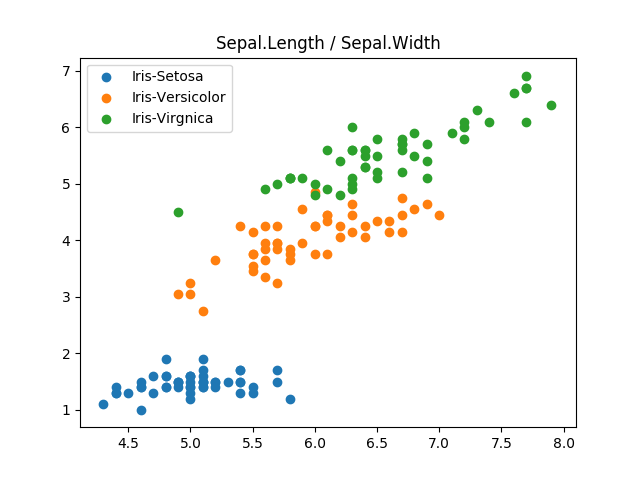
\includegraphics[scale=0.5]{plots/basic_scenario2_cmpnt3.png}
  \captionof{figure}{Standard data set.}
  \label{fig:16}
\end{minipage}
\hfill
\begin{minipage}{0.4\textwidth}
  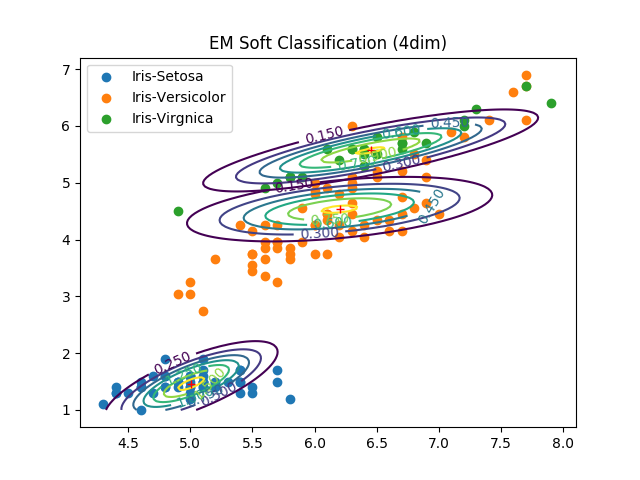
\includegraphics[scale=0.5]{plots/soft_classification_scenario2_cmpnt3.png}
  \captionof{figure}{Gaussian mixture model.}
  \label{fig:17}
\end{minipage}
\end{figure} 

\noindent
Here we used the Expectation Maximization algorithm to learn a gaussian mixture model for a 4-dimensional data set and 3 components. Since the calculation of the initial values for our EM implementation stays the same, the values are chosen randomly between the values of the given data set. To make the outcome comparable to the 2-dimensional outcome we used the same two features (0 and 2) for our plots. Compared to the 2-dim outcome, the \textit{Iris-Setosa} is still classified well, but the classification of \textit{Iris-Versicolor} and \textit{Iris-Virgnica} wasn't that accurate than in the 2-dim data set in our implementation. \\
\newpage
\noindent
{\large \textbf{Comparing with different Component Numbers}} \\

%%%%%%%%%%%%%%%%% Component Numbers %%%%%%%%%%%%%%%%%

\begin{figure}[htp]
\centering
\begin{minipage}{0.4\textwidth}
  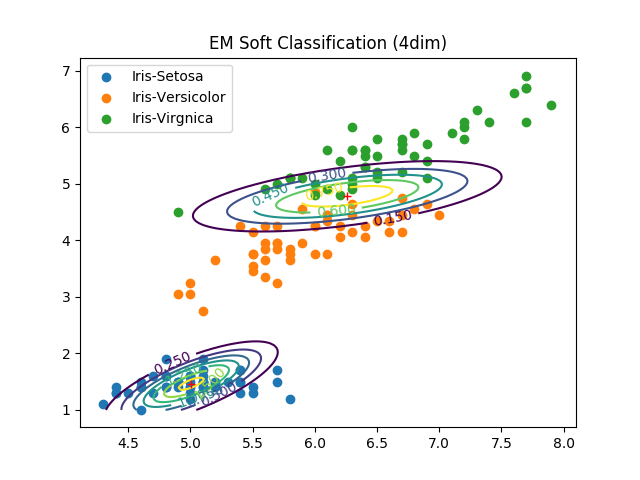
\includegraphics[scale=0.5]{plots/gauss_sc2_c2.png}
  \captionof{figure}{Gaussian mixture model with 2 components.}
  \label{fig:16}
\end{minipage}
\hfill
\begin{minipage}{0.4\textwidth}
  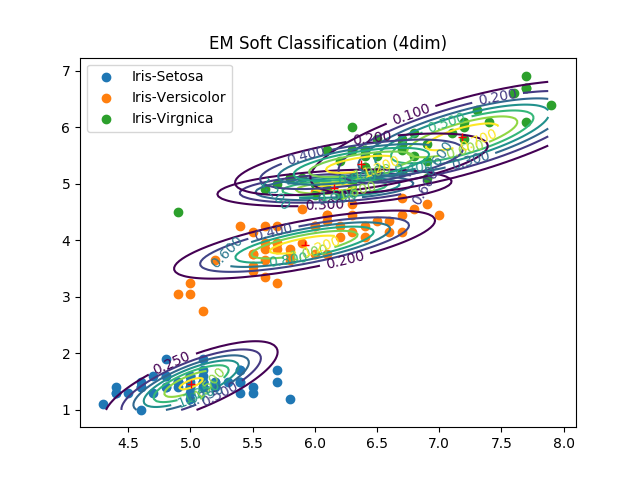
\includegraphics[scale=0.5]{plots/gauss_sc2_c5.png}
  \captionof{figure}{Gaussian mixture model with 5 components.}
  \label{fig:17}
\end{minipage}
\end{figure} 

\noindent
On the right side we have the gaussian mixture model with 2 components where the cluster of the dataset are classified as expected but not that accurate than in D = 2. This may also happen because of the random initial values. Here it could have been useful to use mean dependent initial values to get a more stable result. The plot with the 5 components also classified \textit{Iris-Setosa} perfectly as well, but also classified \textit{Iris-Versicolor} much better than with less components. The \textit{Iris-Virgnica} is classified into 3 different classes. This may also happen because the \textit{Iris-Versicolor} and \textit{Iris-Virgnica} are in the same cluster and if the \textit{Iris-Versicolor} was classified well, so the likelihood is quite good, the other data points are divided into the 3 left over components, compared to the components of the 2dim where the \textit{Iris-Setosa} is split up into two different classes. \\

\noindent
{\large \textbf{Log Likelihood over Iterations}} \\

%%%%%%%%%%%%%%%%% Log Likelihood %%%%%%%%%%%%%%%%%

\begin{figure}[htp]
\centering
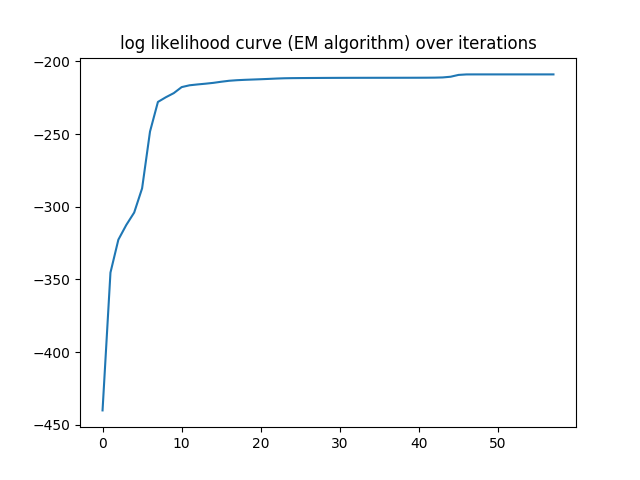
\includegraphics[scale=0.5]{plots/LL_scenario2_cmpnt3.png}
  \captionof{figure}{log-likelihood function over the iterations.}
  \label{fig:17}
\end{figure}

\noindent
This time the sum of the probabilities of the parameters in our data set has a steadier increase than in the 2-dim data set.
As shown in the figure above the log-likelihood is increasing over the numbers of iterations. It doesn't change that much after a certain point of iterations (in our case around 45 iterations) while performing with 150 iterations. In our implementation the local maxima stays around at a value of -210.\newline \newline

\newpage
{\large \textbf{Scatter Plot with Soft Classification}} \\

%%%%%%%%%%%%%%%%% Scatter Plot %%%%%%%%%%%%%%%%%

\begin{figure}[htp]
\begin{minipage}{0.4\textwidth}
	\centering
  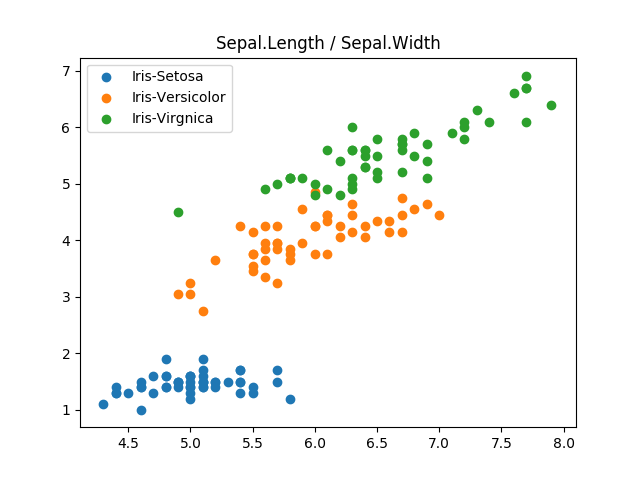
\includegraphics[scale=0.6]{plots/basic_scenario2_cmpnt3.png}
  \caption{Standard data set.}
\end{minipage}
\hfill
\begin{minipage}{0.4\textwidth}
	\centering
  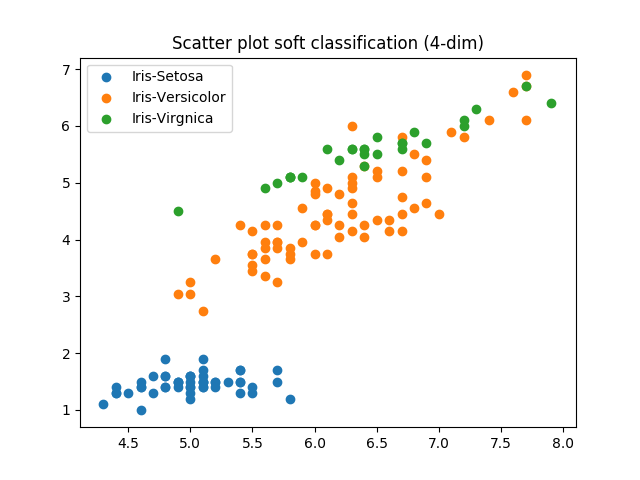
\includegraphics[scale=0.6]{plots/soft_scatter_scenario2_cmpnt3.png}
  \caption{Soft-classification.}
\end{minipage}
\end{figure}

\noindent
In the right plot we can see in detail which points are classified into the classes they belong. Other than the result of the 2-dimensional data set, the classification of the second cluster, including \textit{Iris-Versicolor} and \textit{Iris-Virgnica}, is not that reliable. This effect may occur because of the calculation of the 4-dimensional data set and using only two of their feature when plotting them afterwards. \\

\noindent
{\large \textbf{Comparing Standard Dataset with K-mean Model}} \\

%%%%%%%%%%%%%%%%% K-mean Model %%%%%%%%%%%%%%%%%
  
\begin{figure}[htp]
\centering
\begin{minipage}{0.4\textwidth}
  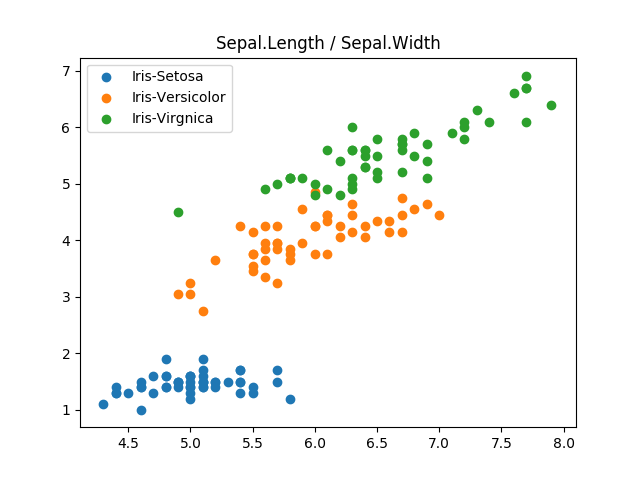
\includegraphics[scale=0.5]{plots/basic_scenario2_cmpnt3.png}
  \captionof{figure}{Standard data set.}
  \label{fig:16}
\end{minipage}
\hfill
\begin{minipage}{0.4\textwidth}
  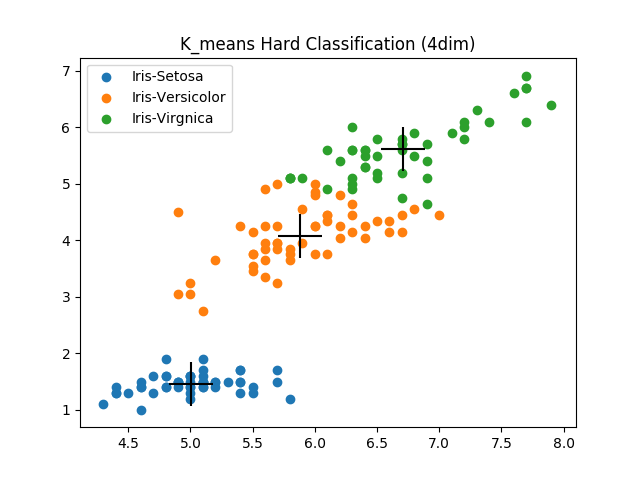
\includegraphics[scale=0.5]{plots/hard_classification_scenario2_cmpnt3.png}
  \captionof{figure}{K-mean model.}
  \label{fig:17}
\end{minipage}
\end{figure}

\noindent
When testing the K-Mean algorithm with three clusters the classification works not as well as it does in 2dim but the centers are almost identical to the 2dim centers.\\

\newpage
{\large \textbf{Comparing with different Component Numbers}} \\

%%%%%%%%%%%%%%%%% Component Numbers %%%%%%%%%%%%%%%%%

\begin{figure}[htp]
\centering
\begin{minipage}{0.4\textwidth}
  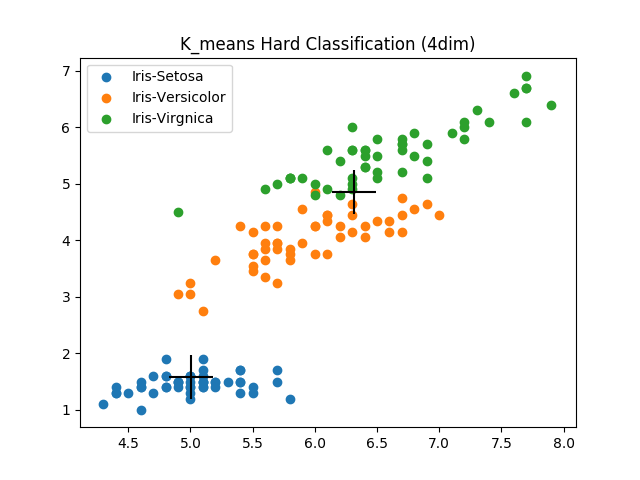
\includegraphics[scale=0.5]{plots/kmeans_sc2_c2.png}
  \captionof{figure}{K-mean model with 2 components.}
  \label{fig:16}
\end{minipage}
\hfill
\begin{minipage}{0.4\textwidth}
  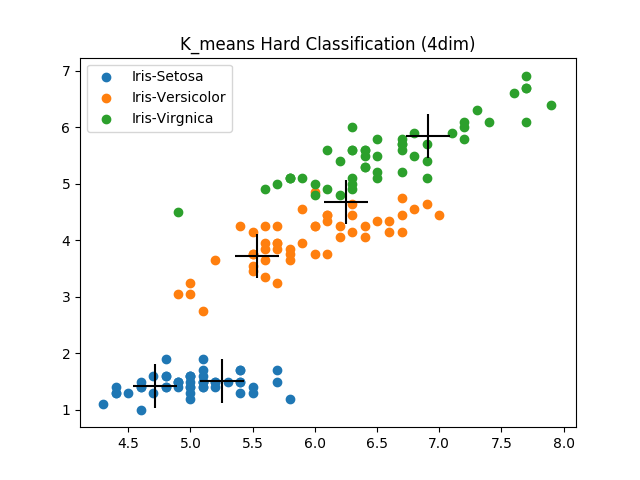
\includegraphics[scale=0.5]{plots/kmeans_sc2_c5.png}
  \captionof{figure}{K-mean model with 5 components.}
  \label{fig:17}
\end{minipage}
\end{figure}

\noindent
Testing the K-Mean algorithm with two \& five clusters in 4dim showed that not only the centers, like it is when using three clusters, but also the classifications are almost identical to the 2dim classifications. The result of the k-mean algorithm strongly depends on the initial value of $\Theta$ which is also depending on the number of components. \\

\noindent
{\large \textbf{Cumulative Distance over Iterations}} \\

%%%%%%%%%%%%%%%%% Cumulative Distance %%%%%%%%%%%%%%%%%

\begin{figure}[htp]
\centering
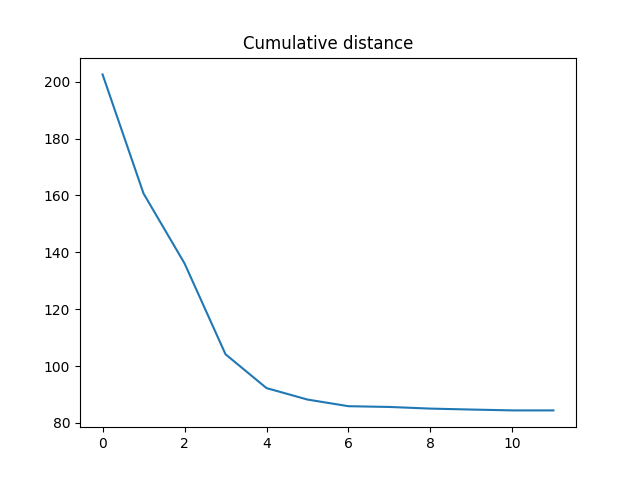
\includegraphics[scale=0.5]{plots/CC_scenario2_cmpnt3.png}
  \captionof{figure}{Cumulative distance over the iterations.}
  \label{fig:17}
\end{figure}

\noindent
As shown in the figure above the cumulative distance is decreasing over the numbers of iterations. The classification in the 4-dim data set with our k-mean found a lot of local minima while using 3 components. After around 10 iterations (while iterating 150 times) the local minima stays steady at a value between 85 and 90. \newline \newline

\newpage
{\large \textbf{Scatter Plot with Hard Classification}} \\

%%%%%%%%%%%%%%%%% Scatter Plot %%%%%%%%%%%%%%%%%

\begin{figure}[htp]
\begin{minipage}{0.4\textwidth}
	\centering
  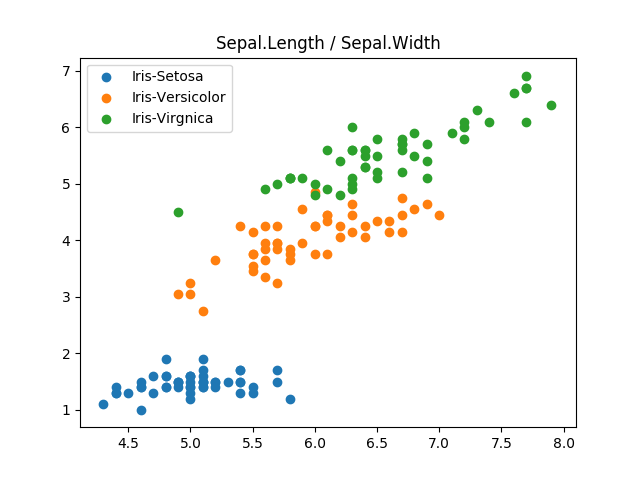
\includegraphics[scale=0.6]{plots/basic_scenario2_cmpnt3.png}
  \caption{Standard data set.}
\end{minipage}
\hfill
\begin{minipage}{0.4\textwidth}
	\centering
  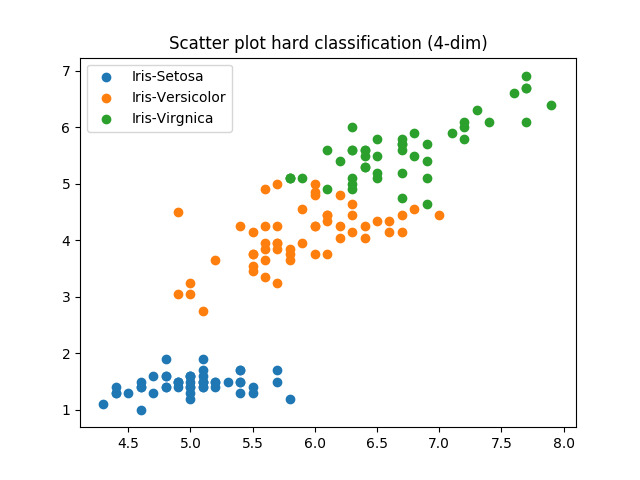
\includegraphics[scale=0.6]{plots/hard_scatter_scenario2_cmpnt3.png}
  \caption{Hard-classification.}
\end{minipage}
\end{figure}

\noindent
The k-mean algorithm in D = 4 performs similar to the k-mean in D = 2 but with slightly better results. \textit{Iris-Setosa} is classified accurate as usual. The difference lies in the classification of \textit{Iris-Virgnica} which now shows a more reliable classification than in the 2-dimensional data set. But this may also occur because of the random initial values.

\begin{enumerate}
\item \textbf{How do the convergence properties and the accuracy of you classification change in comparison to scenario 2.1? [4 Points]} \\ \newline
All in all the convergence properties in the 4-dimensional data set where lower and increased more steady than in the 2-dimensional data set, which also has the effect that the accuracy of the classification is not as reliable as it was in 2dim. But there is also a variance due to the random initializes values used by the EM and K-mean algorithms. \\ \newline
What definitely could be said, is that the k-mean always performs better than the EM algorithm which is used for the Gaussian mixture model.

\newpage

\item \textbf{Within your EM-function confine the structure of the covariance matrices to diagonal matrices! What is the influence on the result. [3 Points]} \\ \newline
Confining the structure of covariance matrices to diagonal ones resulted in the
Gaussian Mixture Model not modeling the data nicely because the Gaussian distribution could only be either stretched horizontally or vertically but not both while the distribution of the data was not that simple. This means that the values of the diagonal matrices are used for the x and y direction of the classification. Since there are no other values expect the diagonal ones there are no values for the rotation of the plotted EM clusters. So they only appear linearly.

\begin{figure}[htp]
\begin{minipage}{0.4\textwidth}
	\centering
  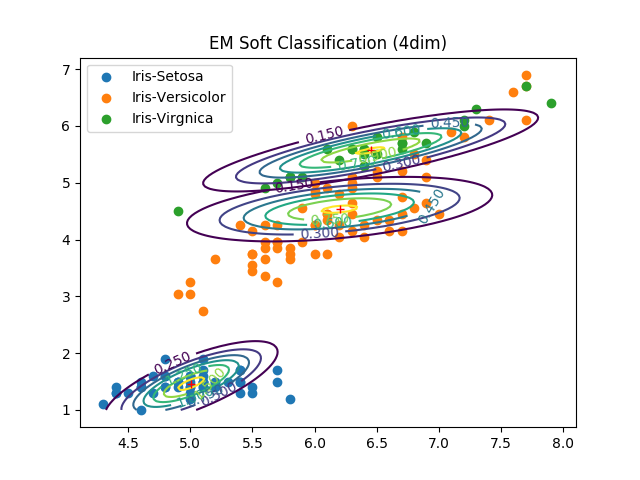
\includegraphics[scale=0.6]{plots/soft_classification_scenario2_cmpnt3.png}
  \caption{Standard structure.}
\end{minipage}
\hfill
\begin{minipage}{0.4\textwidth}
	\centering
  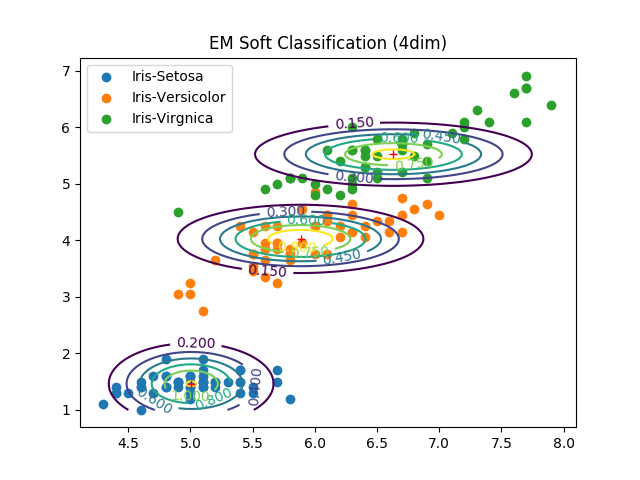
\includegraphics[scale=0.6]{plots/diagonal_4dim.png}
  \caption{Structure with diagonal matrices.}
\end{minipage}
\end{figure}

\end{enumerate}


\newpage
\subsection{Processing the data with PCA [8 + 3* Points]}
Here we perform PCA first to reduce the dimension to $M = 2$ while preserving most of the variance and then apply our algorithms to the transformed data set, i.e., x\_2dim\_pca. \\

\noindent
We implemented the PCA algorithm for reducing the dimension from M = 4 to M = 2 and then applied the EM and the K-mean algorithm. We also used random initial values for our algorithm as already mentioned in the sections above. We first computed the mean vectors of our data and then calculated the covariance matrix depending on the mean vectors calculated before. We extracted the Eigenvectors and Eigenvalues to build up our transformed matrix with a reshape of the Eigenvalues and Eigenvectors, which we then applied to our data set. We also calculated the explained variance of the transformation which is the applied to our transformed data set as a list object. The transformed data set consists of a array (contains transformed data set) and a list with the values of the explained variance. \\

\noindent
{\large \textbf{Comparing PCA Standard Dataset with Gaussian Mixture Model}} \\

%%%%%%%%%%%%%%%%% Gaussian Mixture Model %%%%%%%%%%%%%%%%%
  
\begin{figure}[htp]
\centering
\begin{minipage}{0.4\textwidth}
  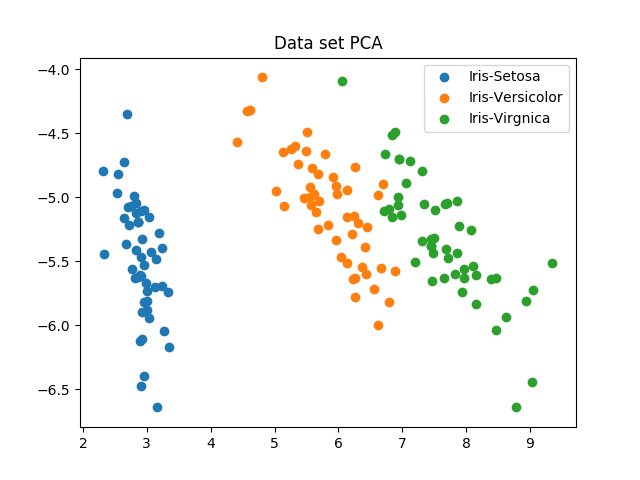
\includegraphics[scale=0.5]{plots/basic_scenario3_cmpnt3.png}
  \captionof{figure}{Standard data set (PCA).}
  \label{fig:16}
\end{minipage}
\hfill
\begin{minipage}{0.4\textwidth}
  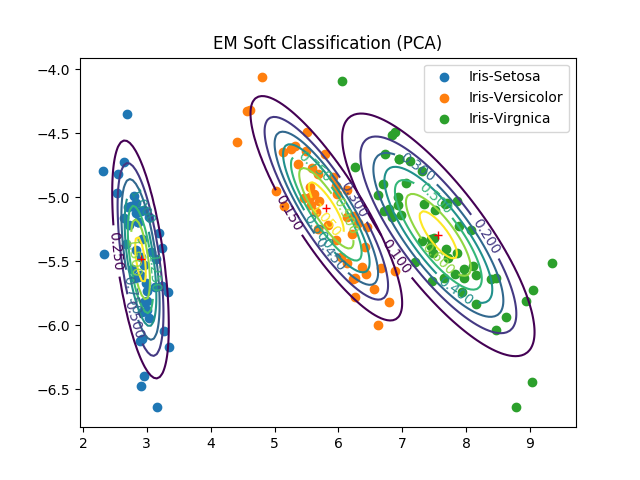
\includegraphics[scale=0.5]{plots/soft_classification_scenario3_cmpnt3.png}
  \captionof{figure}{Gaussian mixture model.}
  \label{fig:17}
\end{minipage}
\end{figure} 

\noindent
The Gaussian mixture model learned by our EM classifies really good the data set transformed by our PCA algorithm. Compared to the 2dim and the 4dim Gaussian mixture model, the EM and K-mean for PCA performs quite good as the 2dim but even much better than our implementation for the 4dimensional data set. We also compared our PCA data set results with already computed PCA for this specific data set and are quite accurate. 

\newpage

{\large \textbf{Comparing with different Component Numbers}} \\

%%%%%%%%%%%%%%%%% Component Numbers %%%%%%%%%%%%%%%%%

\begin{figure}[htp]
\centering
\begin{minipage}{0.4\textwidth}
  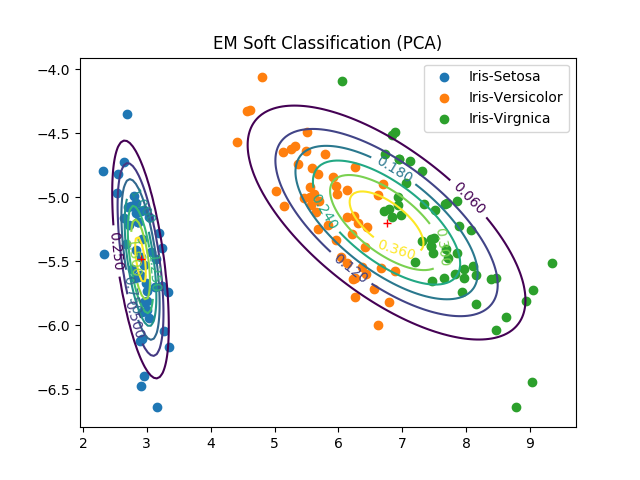
\includegraphics[scale=0.5]{plots/gauss_sc3_c2.png}
  \captionof{figure}{Gaussian mixture model with 2 components.}
  \label{fig:16}
\end{minipage}
\hfill
\begin{minipage}{0.4\textwidth}
  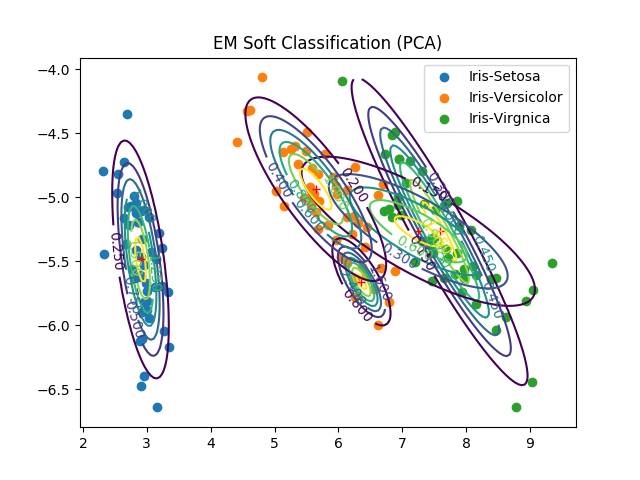
\includegraphics[scale=0.5]{plots/gauss_sc3_c5.png}
  \captionof{figure}{Gaussian mixture model with 5 components.}
  \label{fig:17}
\end{minipage}
\end{figure} 

\noindent
The plot on the left side shows the EM algorithm performed on the PCA data set with 2 components, which is quite accurate since the \textit{Iris-Versicolor} and the \textit{Iris-Virgnica} are classified in same cluster because their data points are quite nearby. The Gaussian mixture model with 5 components splits up the \textit{Iris-Versicolor} and the \textit{Iris-Virgnica} into 4 classes, while the classification of \textit{Iris-Sentosa} with 5 components in the 2dim data set is classified into two different classes, but it performs the same classifications as in the 4dim data set. \\

\noindent
{\large \textbf{Log Likelihood over Iterations}} \\

%%%%%%%%%%%%%%%%% Log Likelihood %%%%%%%%%%%%%%%%%

\begin{figure}[htp]
\centering
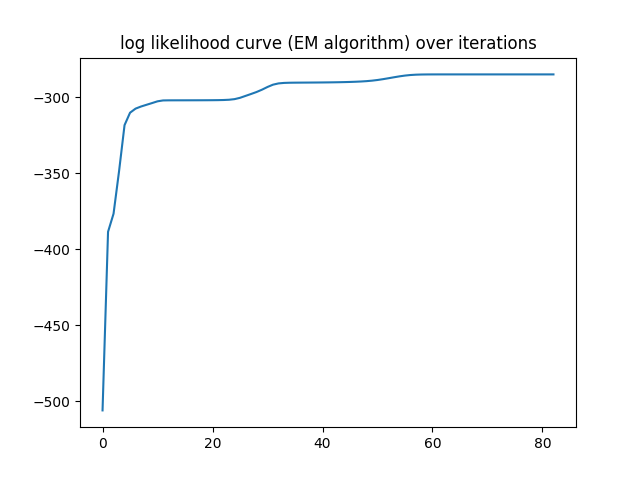
\includegraphics[scale=0.5]{plots/LL_scenario3_cmpnt3.png}
  \captionof{figure}{log-likelihood function over the iterations.}
  \label{fig:17}
\end{figure}

\noindent
In the classification of the PCA data set we got a more fluctuating log-likelihood curve, which means that our probabilities are increasing fast at the beginning but the increase slightly until the convergent point. As shown in the figure above the log-likelihood is increasing over the numbers of iterations. It doesn't change that much after a certain point of iterations (in our case around 55 iterations) while performing with 150 iterations. In our implementation the local maxima stays around at a value of -290.\newline \newline

\newpage

{\large \textbf{Scatter Plot with Soft Classification}} \\

%%%%%%%%%%%%%%%%% Scatter Plot %%%%%%%%%%%%%%%%%

\begin{figure}[htp]
\begin{minipage}{0.4\textwidth}
	\centering
  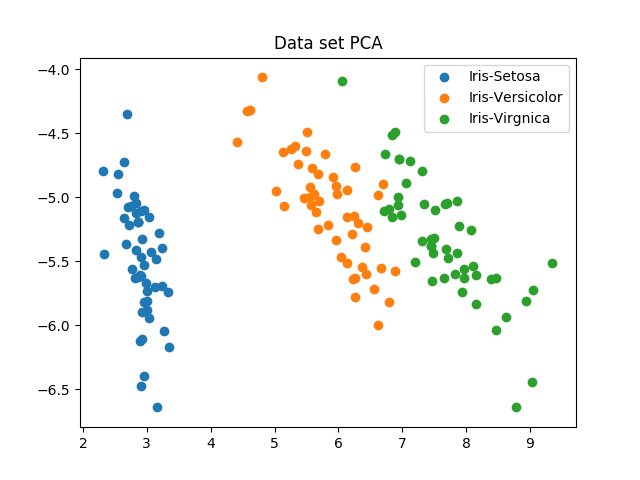
\includegraphics[scale=0.6]{plots/basic_scenario3_cmpnt3.png}
  \caption{Standard data set (PCA).}
\end{minipage}
\hfill
\begin{minipage}{0.4\textwidth}
	\centering
  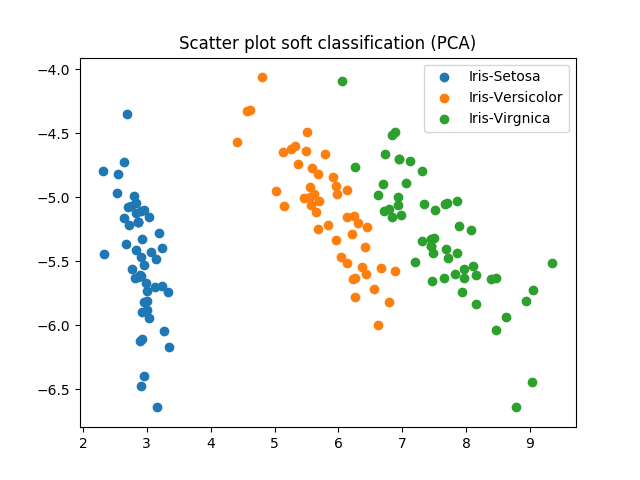
\includegraphics[scale=0.6]{plots/soft_scatter_scenario3_cmpnt3.png}
  \caption{Soft-classification.}
\end{minipage}
\end{figure}

\noindent
The scatter plot shows that the Iris-Setosa cluster classification is as it should be, which means that every data point belonging to the  Iris-Setosa is classified as such. But the Iris-Versicolor looses some points to the Iris-Virgnica. But all in all the soft classification performs similar to the k-mean classification in 2dim \& and 4dim.

\newpage

{\large \textbf{Comparing Standard Dataset with K-mean Model}} \\

%%%%%%%%%%%%%%%%% K-mean Model %%%%%%%%%%%%%%%%%
  
\begin{figure}[htp]
\centering
\begin{minipage}{0.4\textwidth}
  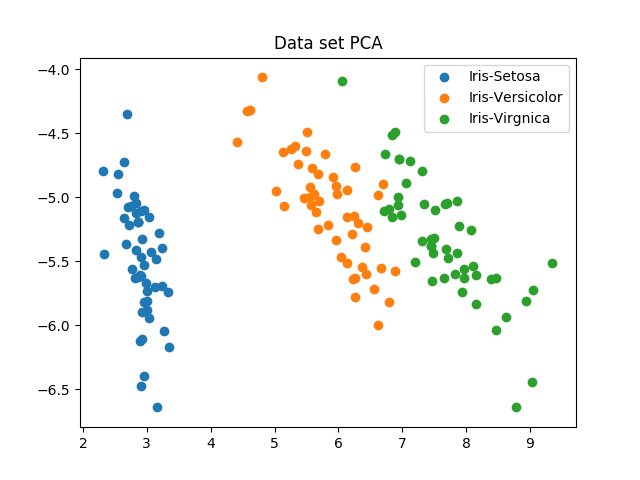
\includegraphics[scale=0.5]{plots/basic_scenario3_cmpnt3.png}
  \captionof{figure}{Standard data set (PCA).}
  \label{fig:16}
\end{minipage}
\hfill
\begin{minipage}{0.4\textwidth}
  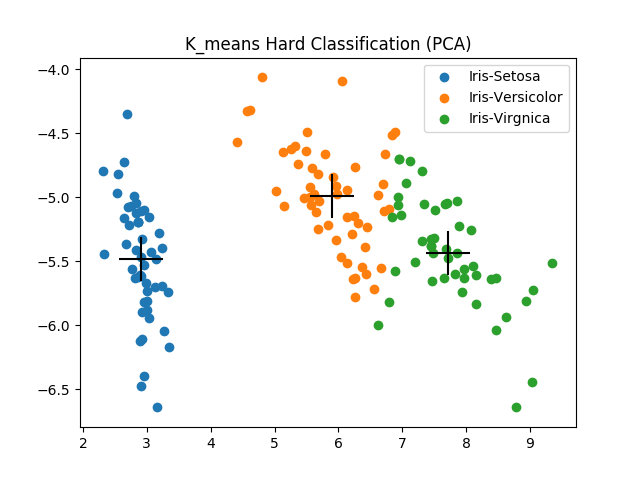
\includegraphics[scale=0.5]{plots/hard_classification_scenario3_cmpnt3.png}
  \captionof{figure}{K-mean model.}
  \label{fig:17}
\end{minipage}
\end{figure}

\noindent
Using the PCA data set and three centers the centers converge to the largest collections of points and the linear classification is very clearly recognizable. \\

\noindent
{\large \textbf{Comparing with different Component Numbers}} \\

%%%%%%%%%%%%%%%%% Component Numbers %%%%%%%%%%%%%%%%%

\begin{figure}[htp]
\centering
\begin{minipage}{0.4\textwidth}
  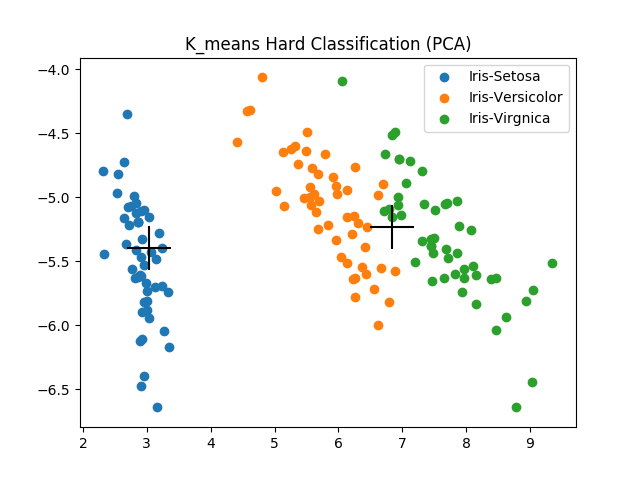
\includegraphics[scale=0.5]{plots/kmeans_sc3_c2.png}
  \captionof{figure}{K-mean model with 2 components.}
  \label{fig:16}
\end{minipage}
\hfill
\begin{minipage}{0.4\textwidth}
  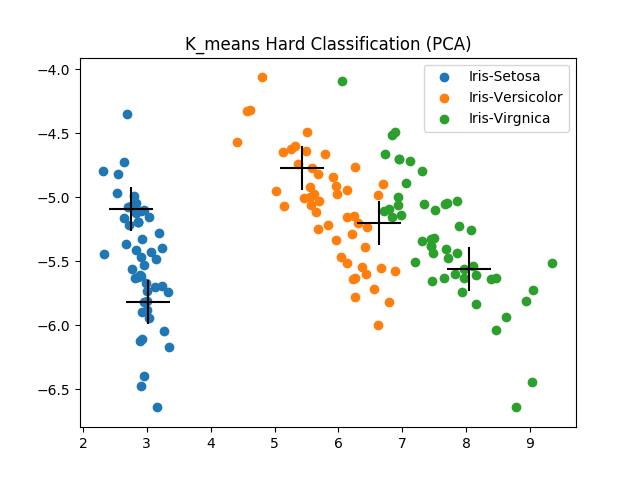
\includegraphics[scale=0.5]{plots/kmeans_sc3_c5.png}
  \captionof{figure}{K-mean model with 5 components.}
  \label{fig:17}
\end{minipage}
\end{figure}

\noindent
Using the PCA data with two \& five clusters showed that when using two clusters, \textit{Iris-Versicolor} \& \textit{Iris-Virgnica} share one center. On the other hand when using 5 clusters, the \textit{Iris-Sentosa} contains two centers, one center is between the \textit{Iris-Virgnica} \& the \textit{Iris-Versicolor} and both the \textit{Iris-Virgnica} \& the \textit{Iris-Versicolor} contain only one center. Also the linear classification isn't as recognizable as it was with three centers. \\

\newpage

{\large \textbf{Cumulative Distance over Iterations}} \\

%%%%%%%%%%%%%%%%% Cumulative Distance %%%%%%%%%%%%%%%%%

\begin{figure}[htp]
\centering
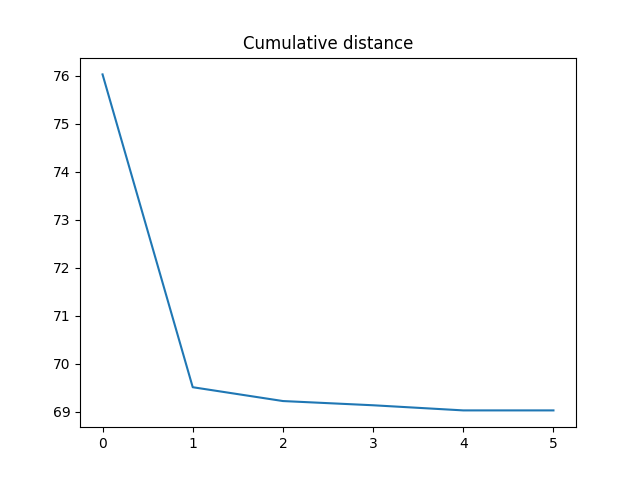
\includegraphics[scale=0.5]{plots/CC_scenario3_cmpnt3.png}
  \captionof{figure}{Cumulative distance over the iterations.}
  \label{fig:17}
\end{figure}

\noindent
As shown in the figure above the cumulative distance is decreasing over the numbers of iterations. The classification in the PCA data set with our k-mean does not found that much of local minima while using 3 components (linear parts). After around 5 iterations (while iterating 150 times) the local minima stays steady at a value of 69. \newline \newline

{\large \textbf{Scatter Plot with Hard Classification}} \\

%%%%%%%%%%%%%%%%% Scatter Plot %%%%%%%%%%%%%%%%%

\begin{figure}[htp]
\begin{minipage}{0.4\textwidth}
	\centering
  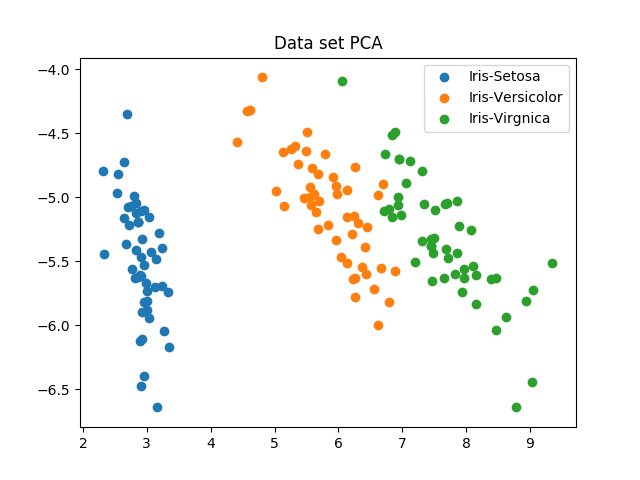
\includegraphics[scale=0.6]{plots/basic_scenario3_cmpnt3.png}
  \caption{Standard data set (PCA).}
\end{minipage}
\hfill
\begin{minipage}{0.4\textwidth}
	\centering
  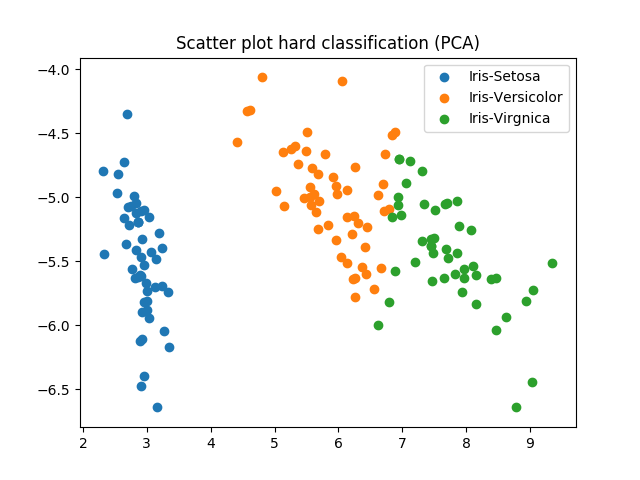
\includegraphics[scale=0.6]{plots/hard_scatter_scenario3_cmpnt3.png}
  \caption{Hard-classification.}
\end{minipage}
\end{figure}

\noindent
The PCA k-mean classification is able to classify most of the components quite well. The Iris-Setosa is perfectly classified whereas the Iris-Versicolor got quite some data from the Iris-Virgnica like it was with the k-mean classification in 4dim. That might be because the k-mean classifies linearly by the distance of the center and so some data of the Iris-Virgnica are closer to the center of the Iris-Versicolor than to the center of Iris-Virgnica. In summary, one can say that the PCA k-mean classification works similar to the 4dim k-mean classification but not as well as the 2dim k-mean classification. \\

\newpage

\begin{enumerate}
\item \textbf{How much of the variance in the data is explained this way? [3 Points]} \\
In total there are 97.67594057574308\% preserved. 92.43644634436244\% in the first \& 5.239494231380641\% in the second dimension. The variance value is appended to our x\_dim2\_pca as a list with 4 values after pca was applied.

\item \textbf{How does the performance of your algorithms compare to scenario 2.1 and scenario 2.2? [5 Points]} \\
The performance of the classification is similar to the 2dim performance but not as good as the 4dim performance which is detailed describes in the plots above.  

\item (bonus-task) Apply PCA with whitening, so that the transformed data has zero mean and a unit covariance matrix. How does this influence the choice of your initialization? [3* Points]
\end{enumerate}

\section*{Samples from a Gaussian Mixture Model [4 Points]}
\begin{enumerate}
  \item Write a function $Y = sample\_GMM(alpha, mu, cov, N)$, that draws $N$ samples from a two-dimensional Gaussian Mixture distribution given by the parameters $alpha$, $mu$ and $cov$!
  \item Using a GMM of your choice $(K > 3)$, demonstrate the correctness of your function!
\end{enumerate}
\end{document}




